
\subsection{Cursor trajectories}


As described in Chapter 2,
cursor transition probabilities were calculated for each condition.
When base rates and descriptions disagreed,
participants initially moved towards
the option cued by the description on 66\% of trials,
selected this option after initially moving towards it 89\% of the time,
and selected the base rate-cued option after
initially moving towards it 36\% of the time.



\subsubsection{Effect of descriptions on base rate choices}




\begin{figure}[ht]
  \begin{floatrow}
    \ffigbox[.5\textwidth]{%
      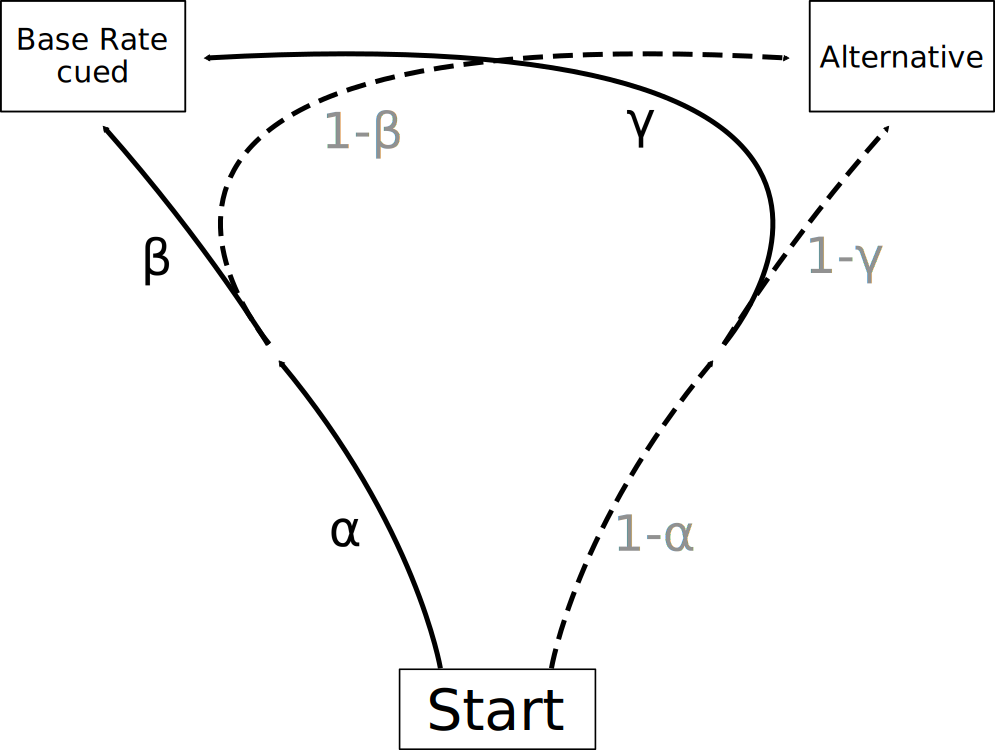
\includegraphics[width=.5\textwidth]{imgs/br_transitions.pdf}
    }{%
      \caption{
        The possible transitions that can occur during a trial
        where the base rate cues a response.
        \label{fig:exp5_br_transitions}
      }
    }
    \capbtabbox{%
      \centering
      \begin{tabular}{llll}
        \toprule
        Description   & $\alpha$ & $\beta$ & $\gamma$\\
        \midrule
        Agreed        & 69.4\%   & 96.5\%  & 89.5\%\\
        Uninformative & 57.4\%   & 79.1\%  & 56.3\%\\
        Disagreed     & 33.8\%   & 36.1\%  & 11.2\%\\
        \bottomrule
      \end{tabular}
    }{%
      \caption[Effect of descriptions on transition probabilities, Experiment 5.]{
        Transition probabilities for trials where the description either
        agreed with the base rate, was uninformative,
        or disagreed with the base rate.
        %% In this analysis $\alpha$ represents the proportion of trials
        %% that initially moved towards the base rate-cued option,
        %% $\beta$ the proportion that select that option
        %% after moving towards it,
        %% and $\gamma$ the proportion who selected the base rated-cued option
        %% after moving towards the alternative.
        There were significant main effects of description type,
        and significant pairwise differences between each description,
        on all measures.
        %% and significant pairwise differences
        %% between each description for all three proportions (p's < .001).
        \label{tab:exp5_br_transitions}
      }%
    }
  \end{floatrow}
\end{figure}



There was a significant main effect of the description type
on the proportion, $\alpha$ of trials where
initially moved towards the base rate-cued option
($\chi^2$ = 135.9, DF = 2, p < .0001).
Participants were most likely to initially move towards
this option
when the description also cued it (69.4\%),
less likely when the description was uninformative (57.4\%)
and least likely when the description cued the alternative option (33.9\%).
Pairwise comparisons between each description type
were all statistically significant
(z's > 3.9, p's < .001).

$\beta$ indicates the proportion of trials
where participants selected the base rate-cued option
after initially moving towards it.
There was a significant main effect of description type on this measure
($\chi^2$ = 262.7, DF = 2, p < .0001).
Participants were most likely to select the base rate-cued option
after initially moving towards it
when the description also cued that option (96.5\% of trials),
less likely when the description was uninformative (79.1\%)
and least likely when the description cued the alternative option (36.1\%).
Pairwise comparisons between each description type
were again all statistically significant
(z's > 5, p's < .0001).


Lastly, $\gamma$ reflects the proportion
of trials where participants selected the base rate-cued option
after initially moving towards the alternative option.
There was a significant main effect of description type
($\chi^2$ = 301.4, DF = 2, p < .0001).
Participants were most likely to change direction
and select the base rate-cued option
after initially moving towards the alternative
when the description agreed with the base rate (89.5\% of trials),
less likely when the description was uninformative (56.3\%),
and were very unlikely to change direction
when that alternative was cued by the description (11.2\%).
Pairwise comparisons between each description type
were once again all statistically significant
(z's > 5, p's < .0001).

These results show that description interfered with
participants' base rate-based reasoning at every juncture,
influencing both their initial mouse movements,
and their subsequent responses,
regardless of their initial movement.


\subsubsection{Effect of base rates on description choices}




\begin{figure}[ht]
  \begin{floatrow}
    \ffigbox[.5\textwidth]{%
      \includegraphics[width=.5\textwidth]{imgs/desc_transitions.pdf}
    }{%
      \caption{
        The possible transitions that can occur during a trial
        where the description cues a response.
        \label{fig:exp5_desc_transitions}
      }
    }
    \capbtabbox{%
      \centering
      \begin{tabular}{llll}
        \toprule
        Base rate     & $\alpha$ & $\beta$ & $\gamma$\\
        \midrule
        Agreed        & 69.4\%   & 96.5\%  & 89.5\%\\
        Uninformative & 68.5\%   & 98.0\%  & 84.1\%\\
        Disagreed     & 66.1\%   & 88.8\%  & 63.7\%\\
        \bottomrule
      \end{tabular}
    }{%
      \caption[Effect of base rates on transition probabilities, Experiment 5.]{
        Transition probabilities for trials where
        the base rate either agreed with the description,
        was uninformative, or disagreed with the description.
        %% In this analysis $\alpha$ represents the proportion of trials
        %% that initially moved towards the description-cued option,
        %% $\beta$ the proportion that select that option
        %% after moving towards it,
        %% and $\gamma$ the proportion who selected the description-cued option
        %% after moving towards the alternative.
        There was no effect of base rate type on $\alpha$.
        $\beta$ and $\gamma$ were both significantly lower
        (that is, participants were less likely to select
        the description-cued option, regardless of initial movement direction)
        when the base rate disagreed with the description.
        \label{tab:exp5_desc_transitions}
      }%
    }
  \end{floatrow}
\end{figure}



The transition probability analysis was repeated
to explore the effect of manipulating the base rate
on participants' movements towards the description-cued option.
Transition probabilities,
broken down according to the base rate,
are shown in Table~\ref{tab:exp5_desc_transitions}.
Here, $\alpha$ represents the proportion of trials
where participants initially moved towards the description-cued option.
There was no main effect of base rate on this proportion
($\chi^2$  = 1.5, DF = 2, p > .4):
participants initially moved towards the description-cued option
on average 68\% of the time,
regardless of the base rate information.

There were, however, main effects of base rate type
on $\beta$, the proportion of trials where
the description-cued option was selected after
participants initially moved towards it,
and $\gamma$, the proportion of trials where
the it  was selected after
participants initially moved towards the alternative option
($\chi^2$s  > 30, DF = 2, p's < .0001).
In both cases, participants were less likely
to ultimately select the description-cued option
when the base rate cued the other response option
than when the base rate was uninformative
or when it agreed with the description
(z's > 3, p's < .001; see Table~\ref{tab:exp5_desc_transitions}).

Therefore, base rates had no early impact on participants'
description-based reasoning,
and did not influence their initial mouse movements.
They showed some effect, however, on ultimate responses,
as participants were less likely to select the description-cued option,
regardless of what direction they initially moved the cursor.
